\documentclass{article}
\usepackage{graphicx}

\title{CMSC 6950 - argopy: A Python library for Argo ocean data analysis}
\author{Michael King}

\begin{document}
\maketitle

\section{Introduction}

The objective of this project was to select an open source software package and perform computational tasks using data obtained from a package of choice. The scientific package chosen for my project is called argopy (Maze and Balem, 2020). argopy is a Python library that can be used to download, analyze and interpret ocean data collected by Argo floats. In particular, the argopy Python library permits users to obtain Argo float measurements from Argo floats worldwide that measure pressure, temperature and salinity of the worlds oceans from the surface to 2000m depth every 10 days. Traditionally, the large number of files, data variables and use of jargon associated with the Argo dataset often accompanied a challenging workflow, especially for new users. The motivation of argopy was to provide a Python friendly library where Argo float data can be easily accessible and readable for users who are new to and/or experts with Argo float data. For this project, two computational tasks have been carried out using data extracted from the argopy Python library and other Python modules such as numpy, pandas, geopandas and matplotlib. 

    

\section{Results}

Herein, the results for each computational task will be presented. The first computational task will focus on visualizing the position of Argo floats in a region southeast of Florida and how the total number of floats changes each year. The second computational task is used to visualize the trajectory and temperature variation of two Argo floats with time since the float's deployment.

\subsection{Task 1- Total Argo float numbers through time}

The objective for my first computational task was to retrieve Argo data collected from 2001 to 2006 using argopy and use this data to visualize the change in the total number of Argo floats per year within a region of the Atlantic Ocean, southeast of Florida, USA. This process began by using the ArgoDataFetcher to retrieve Argo data within user specified coordinates for a user specified time frame (2001-01-01 to 2006-12-31). Following this step, the downloaded Argo data (stored as an xarray.Dataset) was converted into a Pandas dataframe, which was then exported as a csv file that served as the intermediate file to perform this computational task. Next, this csv file was loaded into a python script as a Pandas dataframe in order to begin the final data filtering and plotting. Prior to plotting, the original Pandas dataframe was split into 6 different dataframes so that each dataframe contained data only from a certain year from 2001 to 2006. Each dataframe containing Argo data from 2001 to 2006 was then appended to the dataframe of its subsequent year in order to calculate the total number of Argo floats present each year. For example, the dataframe for additional Argo floats deployed in 2002 (400) was appended to the total in 2001 (33) to get the total over those two years (433).Following the completion of data filtering, the matplotlib and geopandas Python libraries were used to plot the position and total number of Argo floats per year with the addition of a base map of North America on each plot (extracted using a dataframe obtained from geopandas) for spatial reference.

\begin{figure}
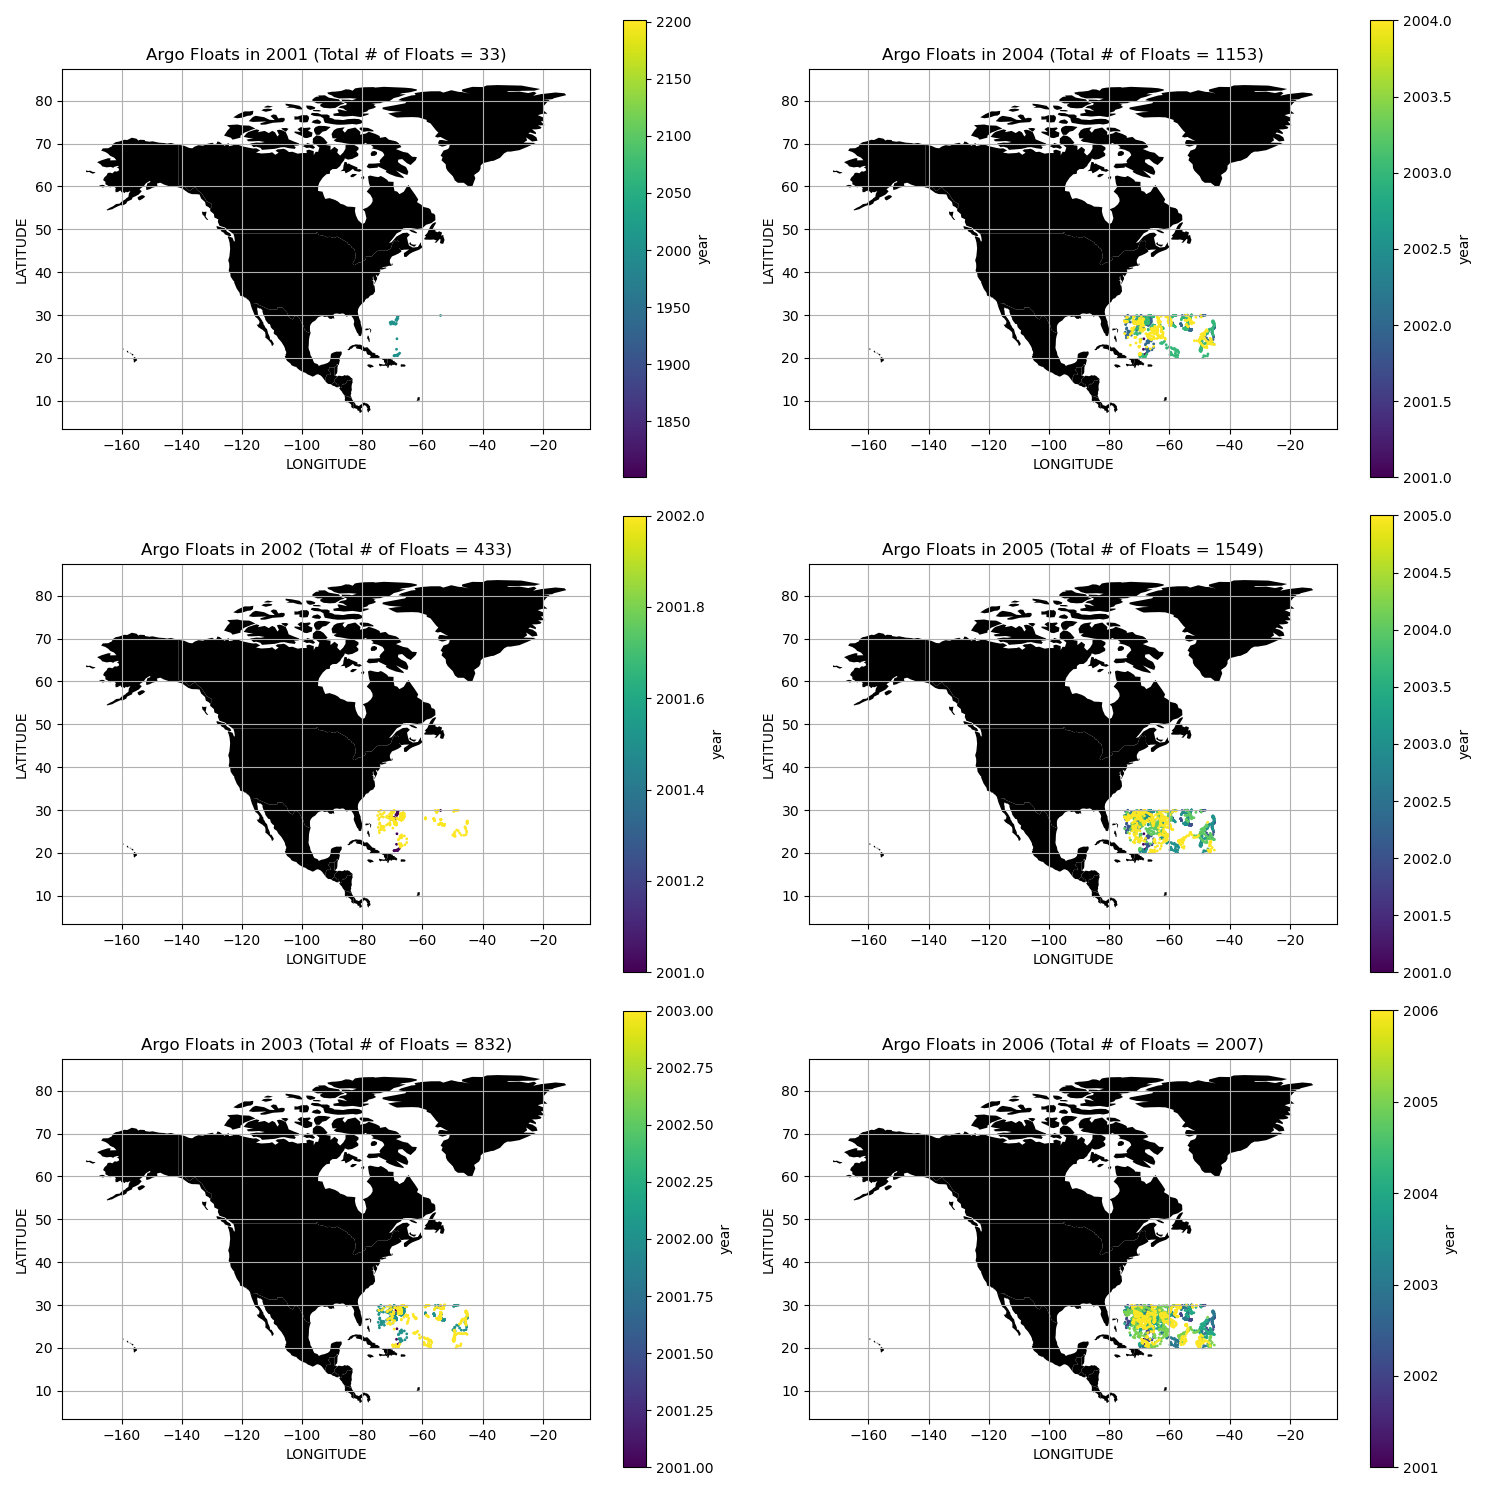
\includegraphics[width=\textwidth,height=\textheight,keepaspectratio]{total_argo.png}
\caption{Total Argo floats for each year from 2001 to 2006 in a region southeast of Florida.}
 
\end{figure}


\subsection{Task 2 - Argo float trajectories}

Show the plot

\begin{figure}[!ht]
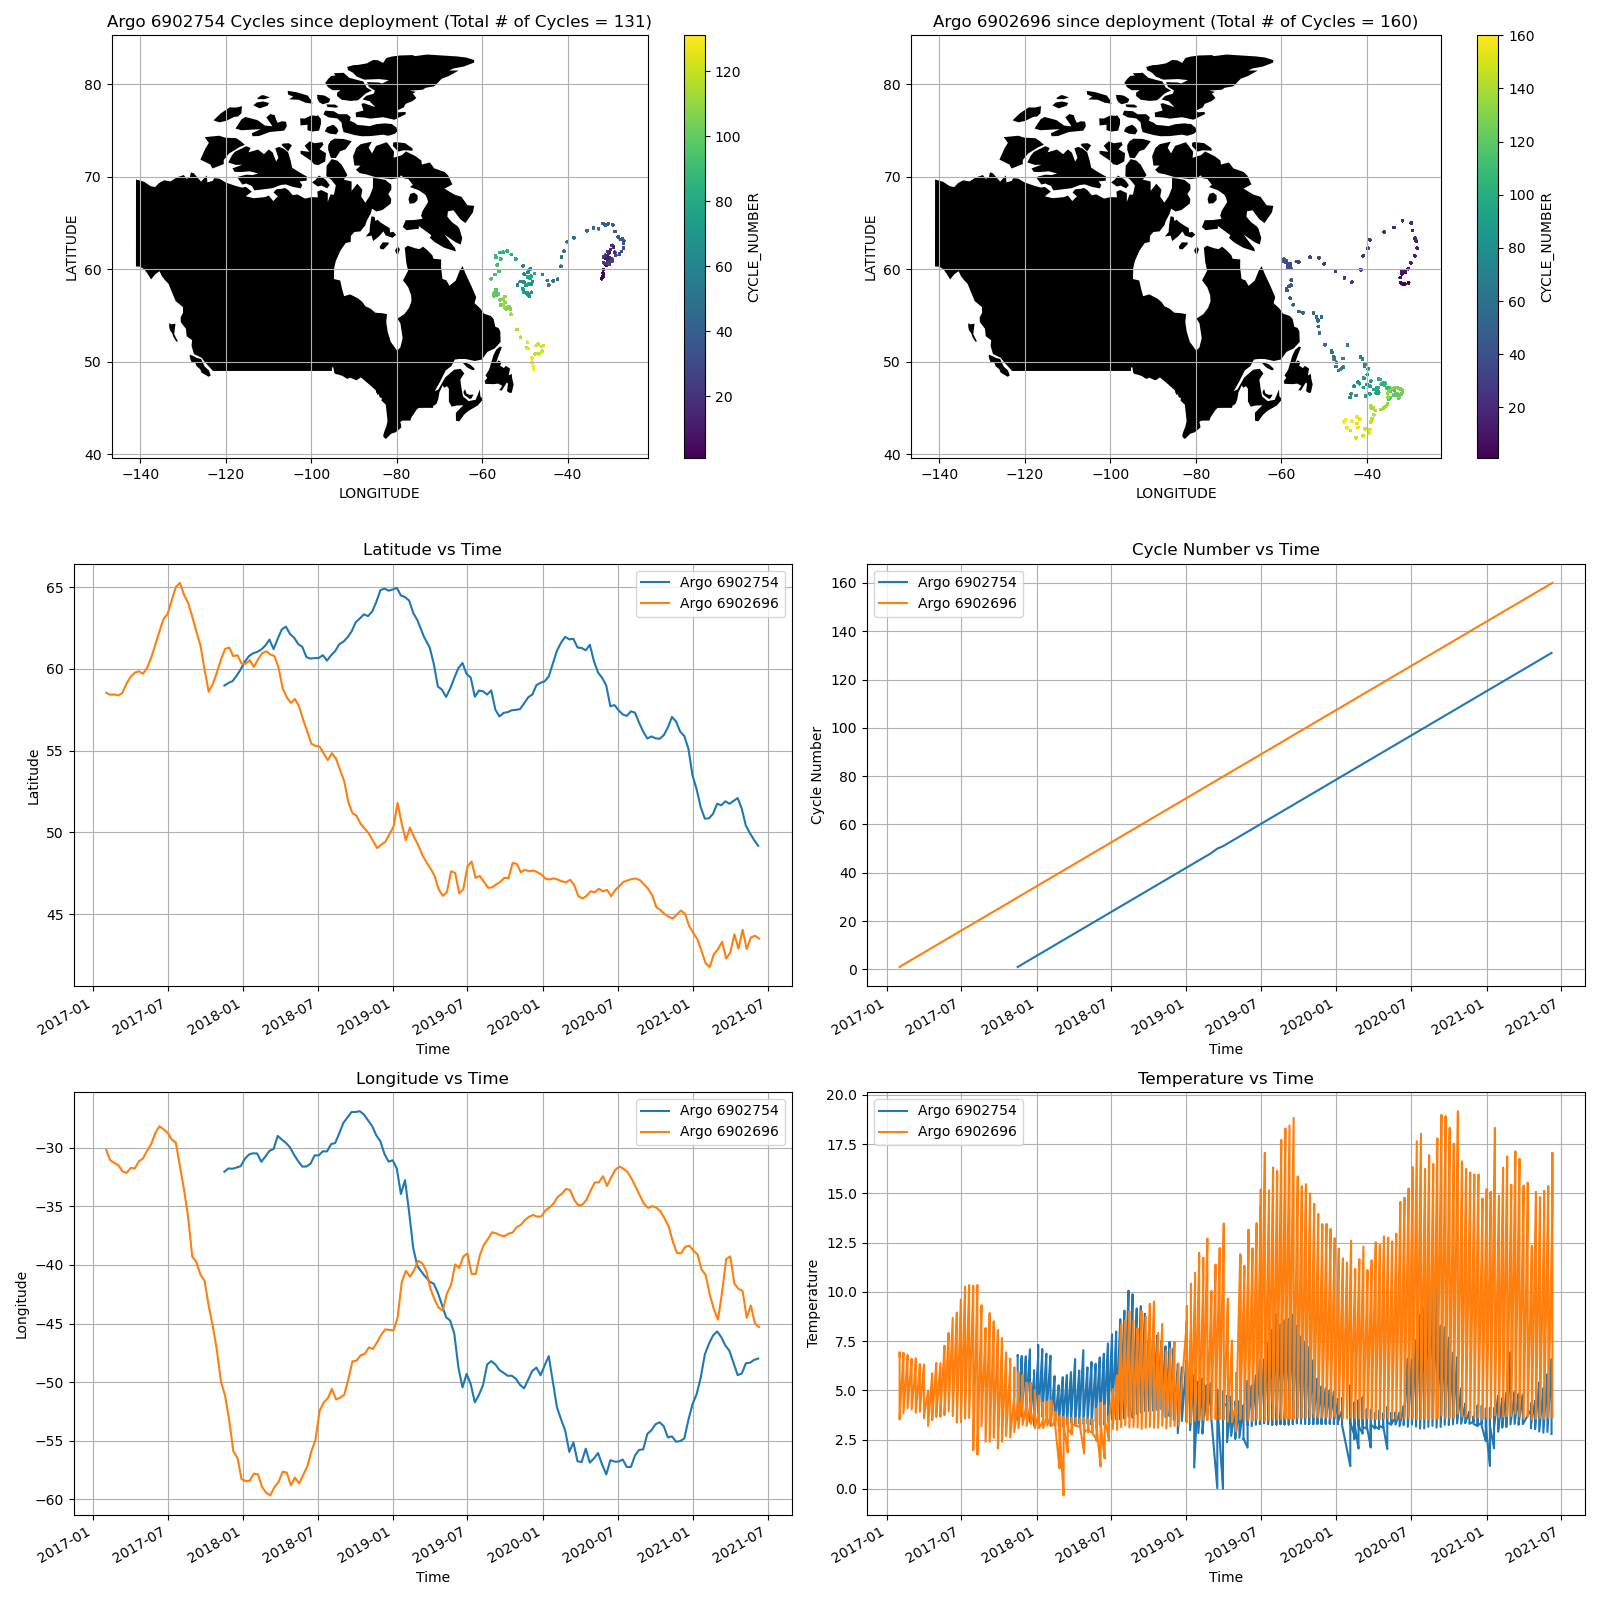
\includegraphics[width=\textwidth,height=\textheight,keepaspectratio]{argo_trajectory.png}
\caption{Trajectory and temperature variation with time of two Argo floats located within the Atlantic Ocean, offshore Newfoundland and Labrador.}
\end{figure}
 
 

\section{Conclusions}

\section{References}

Maze, G., and Balem, K. (2020). argopy: A Python library for Argo ocean data analysis. Journal of Open Source Software, 5(33).

\end{document}